\documentclass[main.tex]{subfiles}
%\graphicspath{{\subfix{../images/}}}
\begin{document}
\begin{enumerate}[label=\textbf{\alph*)}]
    \item O método usado foi o de Runge-Kutta por sue superioridade em relação aos outro dois métodos, como mostrado na questão anterior. O passo utilizado foi de 0.01, um pouco menor do que utilizado anteriormente, com o objetivo de
    tentar aumentar um pouco a precisão, já que esta mudança não afeta o tempo de execução do programa. Outra mudança em relação à questão 1 foi o tempo de execução de 5 período para 15 para se ver mais pontos na seção de Poincaré.
    \item Os gráficos das trajetórias no espaço de fase são:
    \begin{center}
        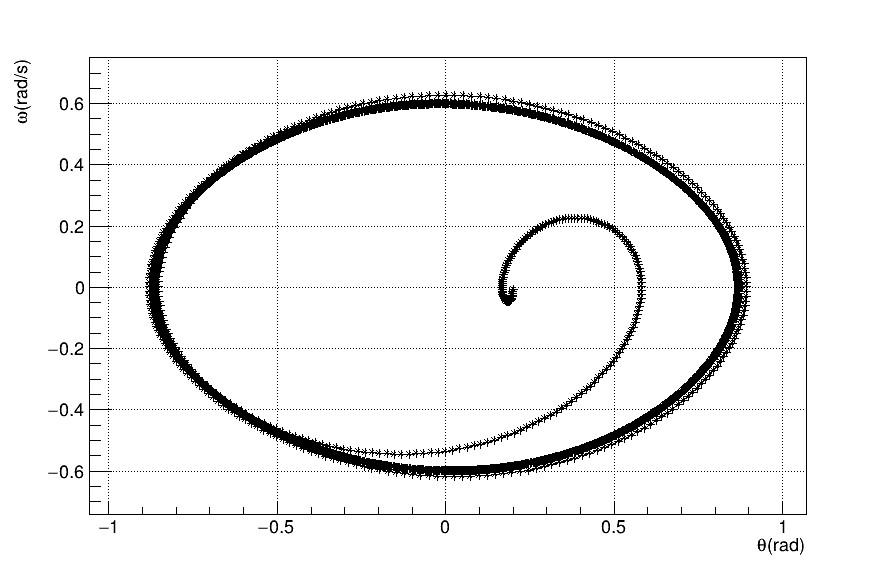
\includegraphics[scale=0.15]{../q2/alpha0.5/plots/theta_omega_RK.png}
        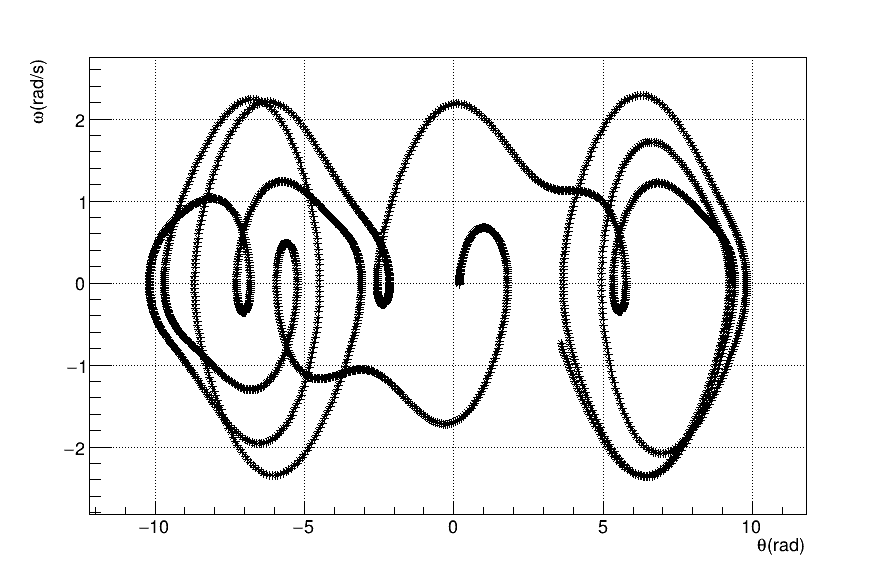
\includegraphics[scale=0.15]{../q2/alpha1.2/plots/theta_omega_RK.png}
        \captionof{figure}{Órbita no espaço de fase para valores de $\alpha = 0.5$ (figura da esquerda) e $\alpha = 1.2$ (figura da direita) produzidos com o método de Runge-Kutta.}
    \end{center}
    \item As seções de Poincaré com a configuração da questão estão nos gráficos abaixo.
    \begin{center}
        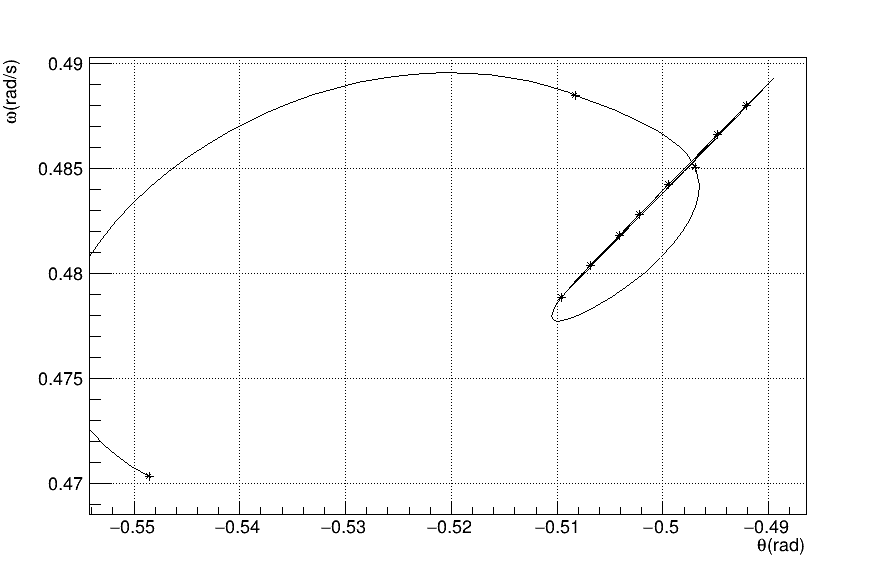
\includegraphics[scale=0.15]{../q2/alpha0.5/plots/poincare_RK.png}
        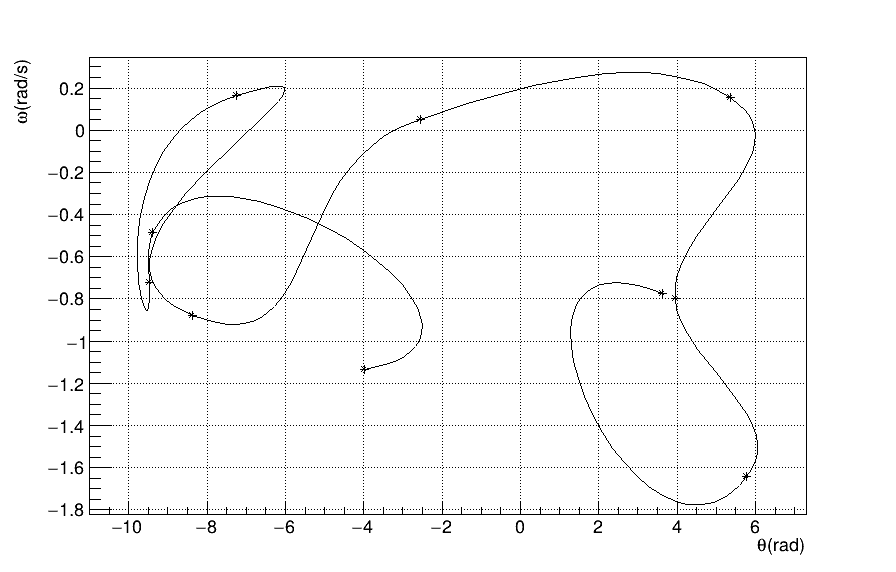
\includegraphics[scale=0.15]{../q2/alpha1.2/plots/poincare_RK.png}
        \captionof{figure}{Seções de Poincaré para valores de $\Omega_D = 2/3$ e $\alpha = 0.5$ (figura da esquerda) e $\alpha = 1.2$ (figura da direita) produzidos com o método de Runge-Kutta.}

    \end{center}
    \item As seções de Poincaré com a $\Omega_D = \frac{4}{3}$ para aparecerem mais ponto na seção.
    \begin{center}
        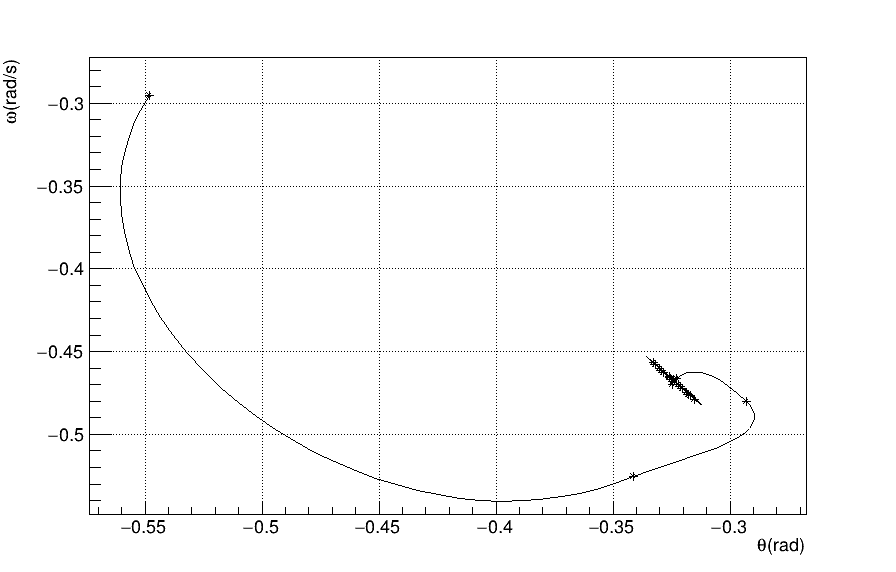
\includegraphics[scale=0.15]{../q2/itemd/alpha0.5/plots/poincare_RK.png}
        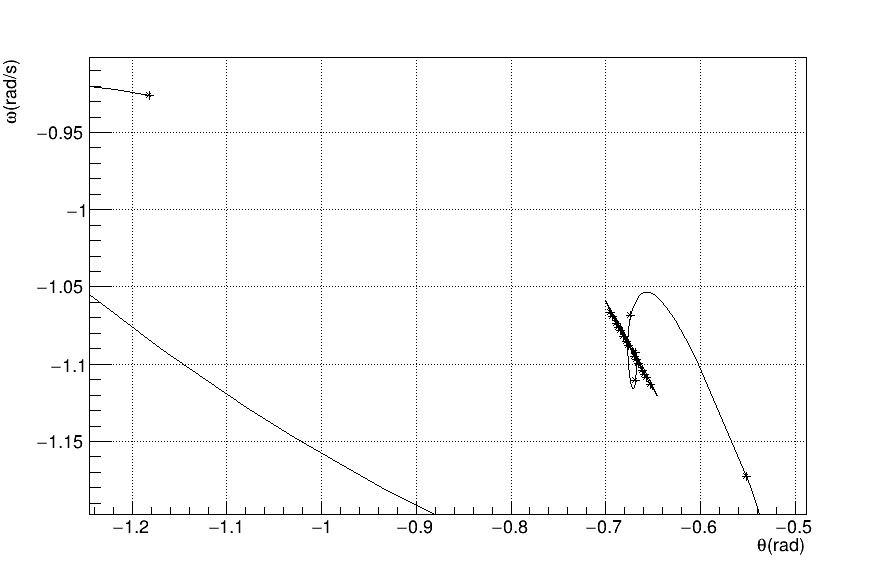
\includegraphics[scale=0.15]{../q2/itemd/alpha1.2/plots/poincare_RK.png}
        \captionof{figure}{Seções de Poincaré para valores de $\Omega_D = 4/3$ e $\alpha = 0.5$ (figura da esquerda) e $\alpha = 1.2$ (figura da direita) produzidos com o método de Runge-Kutta.}
    \end{center}
    \item As seções de Poincaré fornecem uma maneira mais "simples" de se estudar o espaço de fase. Mudando um espaço complicado como do item (b) para um espaço com menos ponto como o do item (c). Além disso, pode-se ver quando
    um movimento converge ou está em um movimento caótico. Abaixo colocarei os gráficos de $\theta \times t$ das seções de Poincaré com $\alpha = 1.2$ mas com $\Omega_D = 2./3$ pro gráfico a esquerda e $\Omega_D = 4./3$ pro gráfico á direita.
    Pode-se ver nas seções de Poincaré que a órbita do item (c) (gráfico à direita) parece convergir, com valores de $\theta$ muito próximos a cada período. Já a órbita do item (b) parece estar menos ordenada.
    \begin{center}
        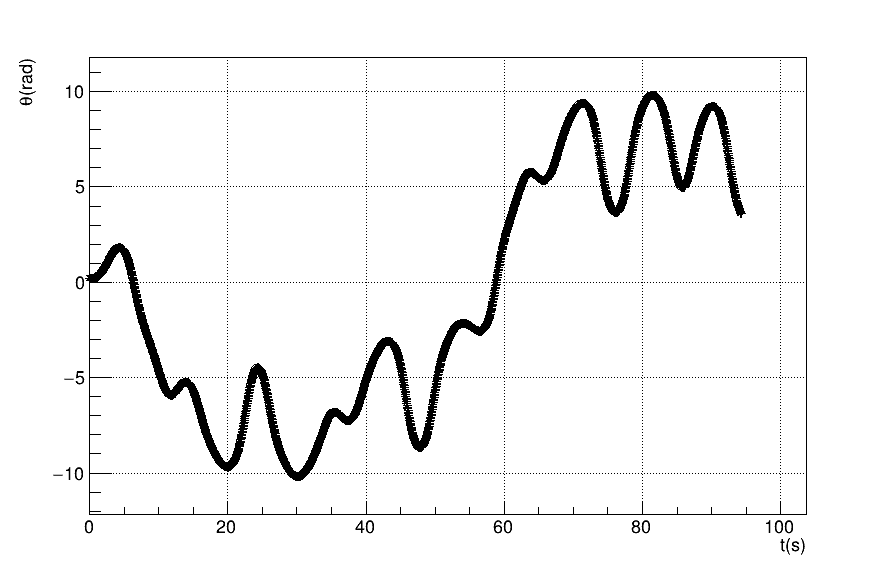
\includegraphics[scale=0.15]{../q2/alpha1.2/plots/theta_t_RK.png}
        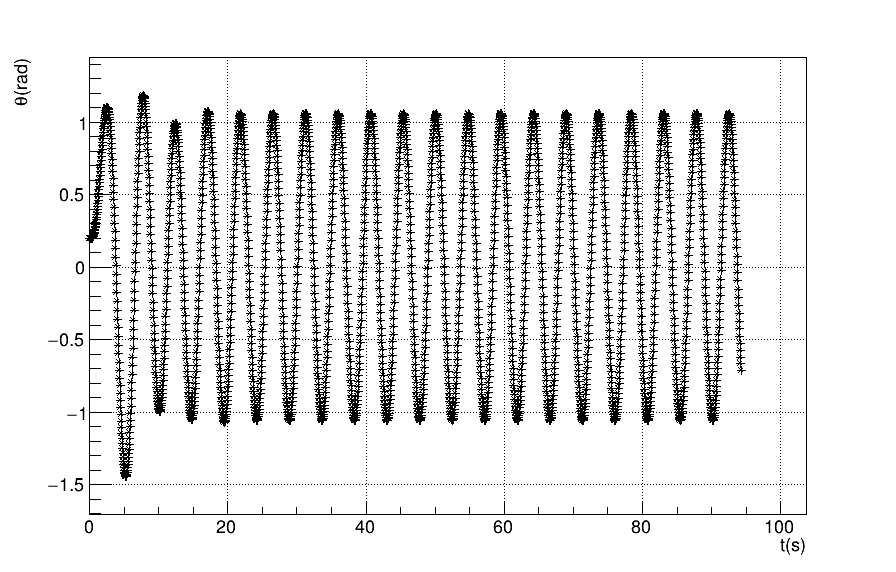
\includegraphics[scale=0.15]{../q2/itemd/alpha1.2/plots/theta_t_RK.png}
        \captionof{figure}{Gráfico de $\theta \times t$ para as seções de Poincaré para valores de $\alpha = 1.2$ e $\Omega_D = 2/3$ (figura da esquerda) e $\Omega_D = 4/3$ (figura da direita) produzidos com o método de Runge-Kutta.}
    \end{center}
\end{enumerate}

\end{document}
% \documentclass[main.tex]{subfiles}
% %\graphicspath{{\subfix{../images/}}}
% \begin{document}
% \begin{center}
%     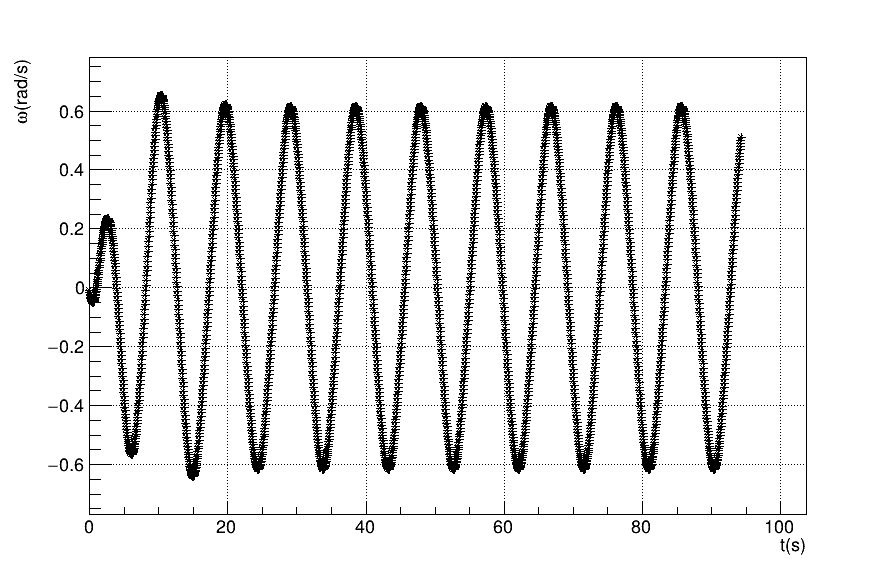
\includegraphics[scale=0.15]{../q2/alpha0.5/plots/omega_t_euler.png}
%     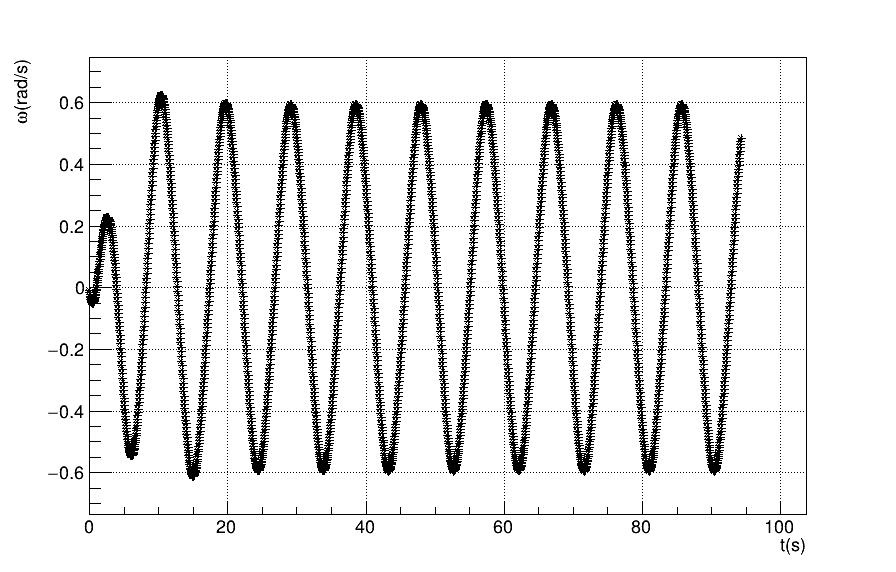
\includegraphics[scale=0.15]{../q2/alpha0.5/plots/omega_t_ec.png}
%     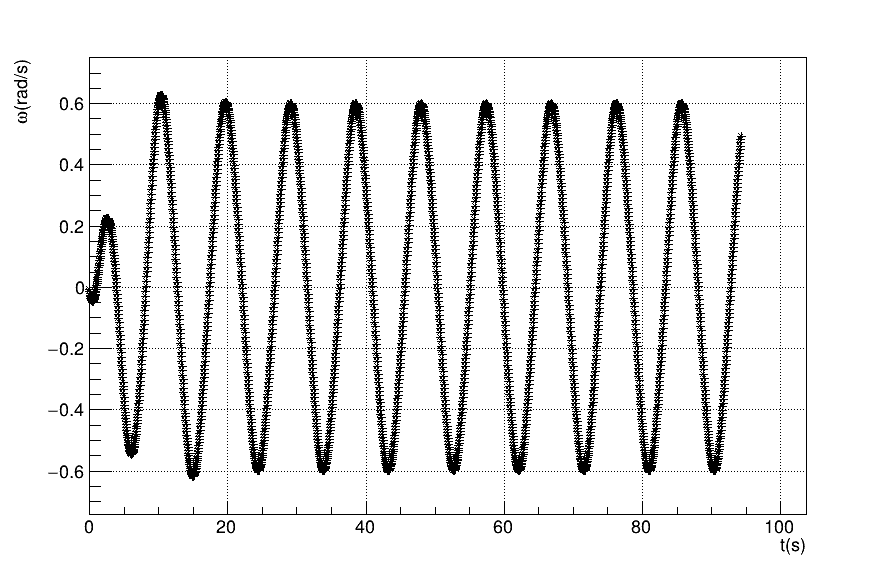
\includegraphics[scale=0.15]{../q2/alpha0.5/plots/omega_t_RK.png}
% \end{center}
% \begin{center}
%     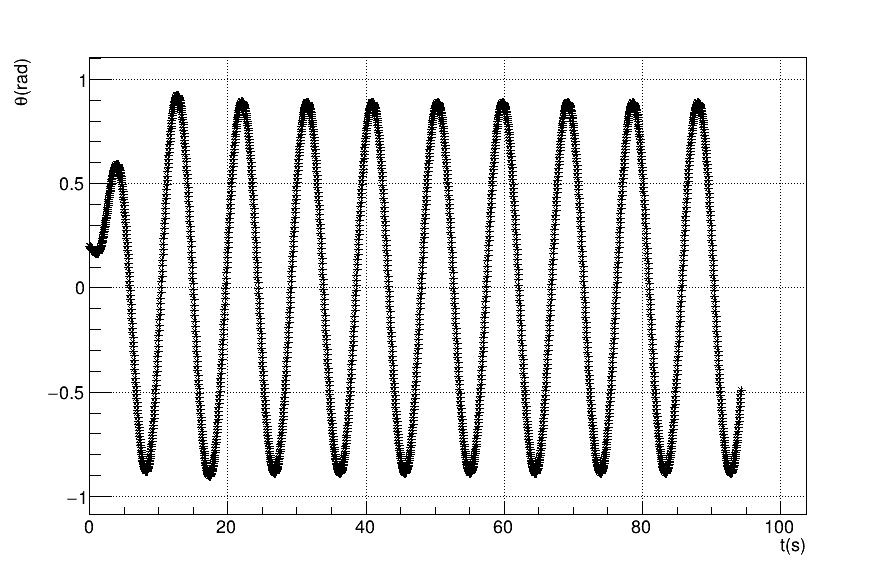
\includegraphics[scale=0.15]{../q2/alpha0.5/plots/theta_t_euler.png}
%     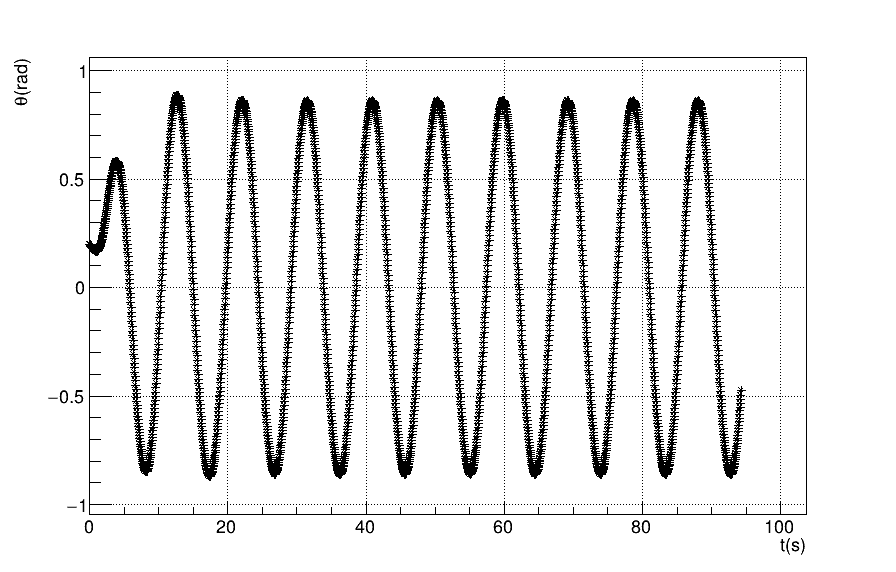
\includegraphics[scale=0.15]{../q2/alpha0.5/plots/theta_t_ec.png}
%     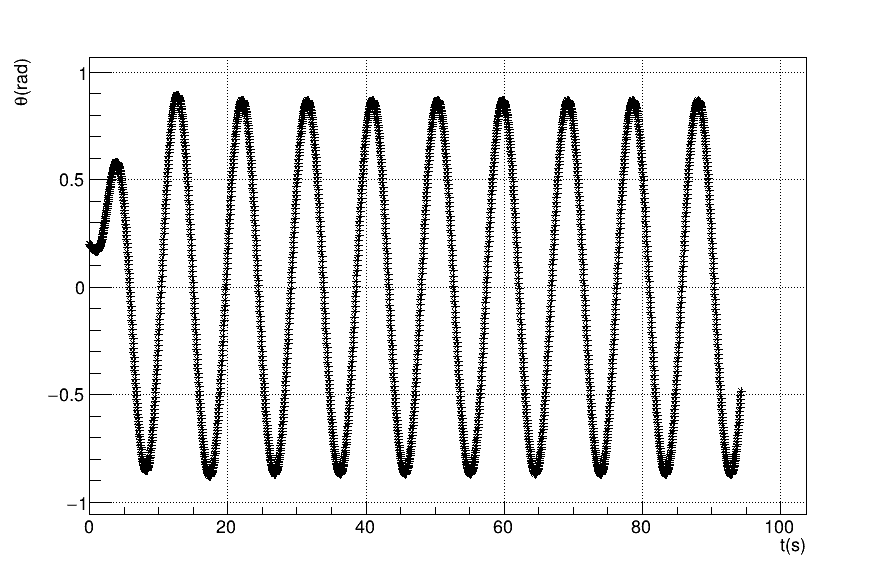
\includegraphics[scale=0.15]{../q2/alpha0.5/plots/theta_t_RK.png}
% \end{center}
% \begin{center}
%     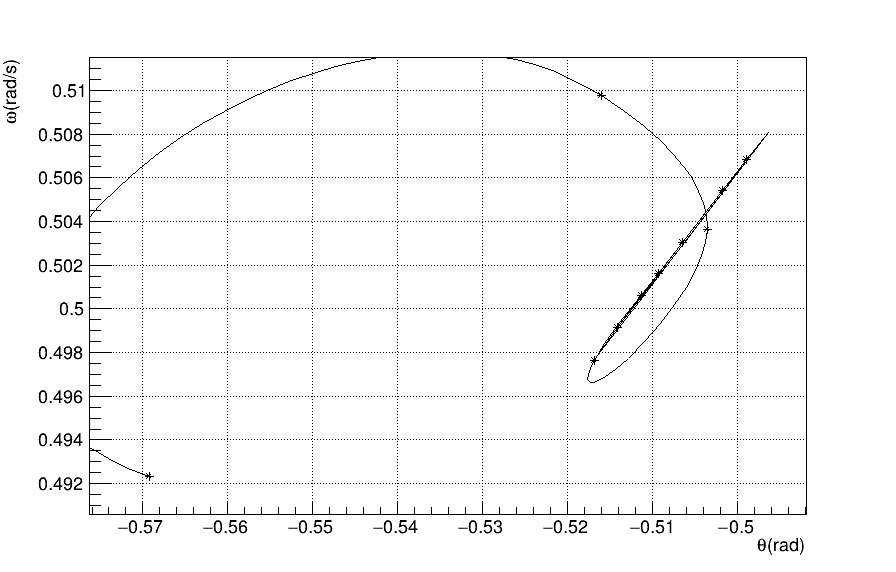
\includegraphics[scale=0.15]{../q2/alpha0.5/plots/poincare_euler.png}
%     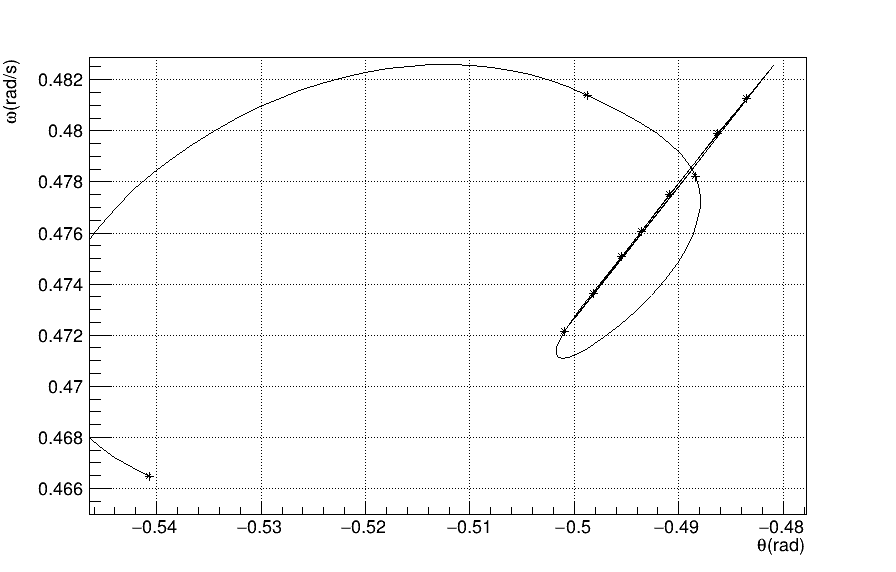
\includegraphics[scale=0.15]{../q2/alpha0.5/plots/poincare_ec.png}
%     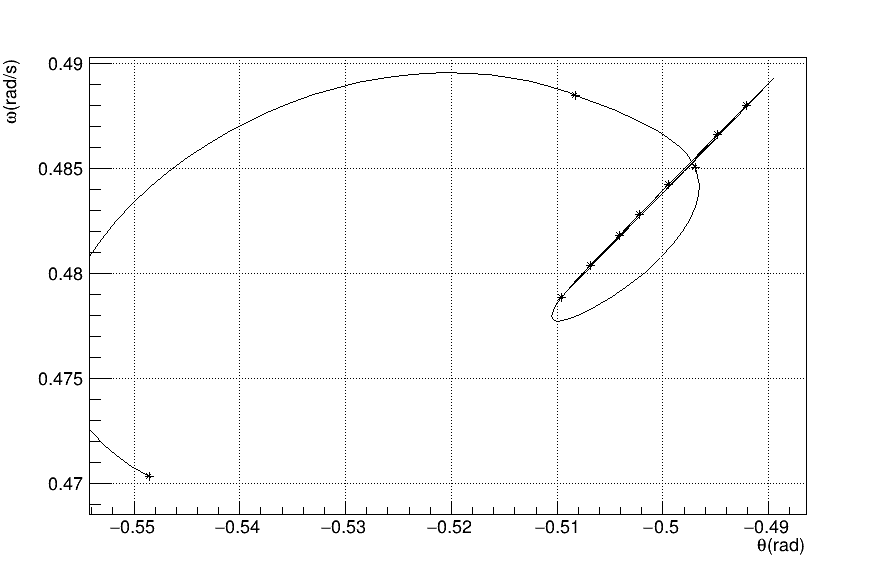
\includegraphics[scale=0.15]{../q2/alpha0.5/plots/poincare_RK.png}
% \end{center}
% \begin{center}
%     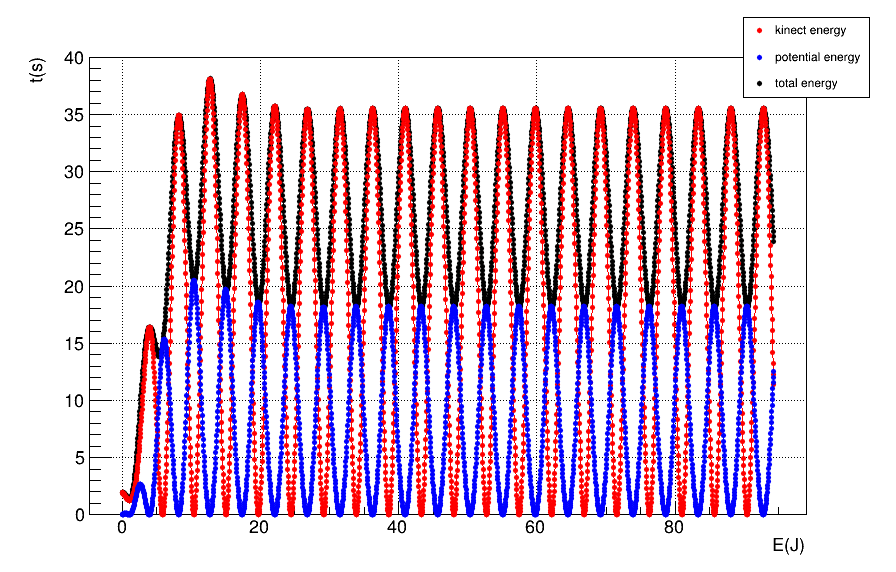
\includegraphics[scale=0.15]{../q2/alpha0.5/plots/Energies_t_euler.png}
%     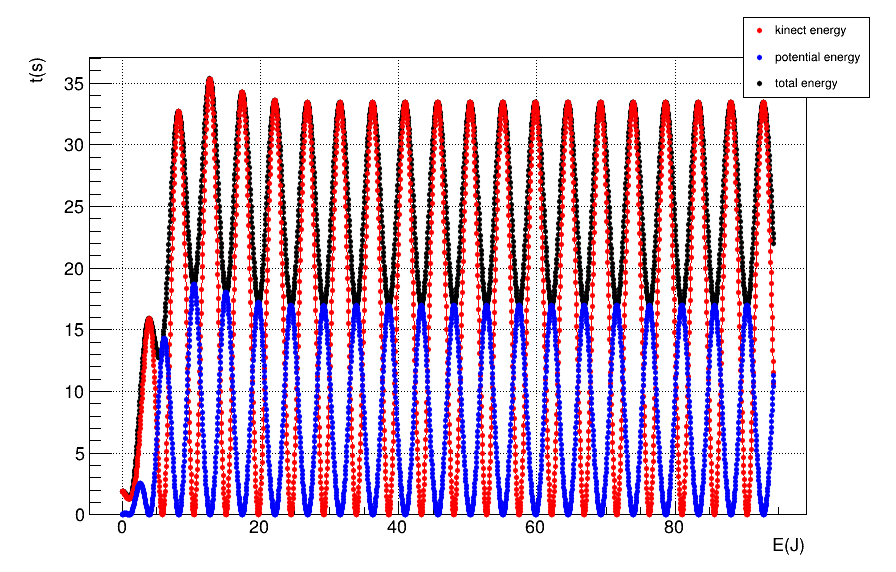
\includegraphics[scale=0.15]{../q2/alpha0.5/plots/Energies_t_ec.png}
%     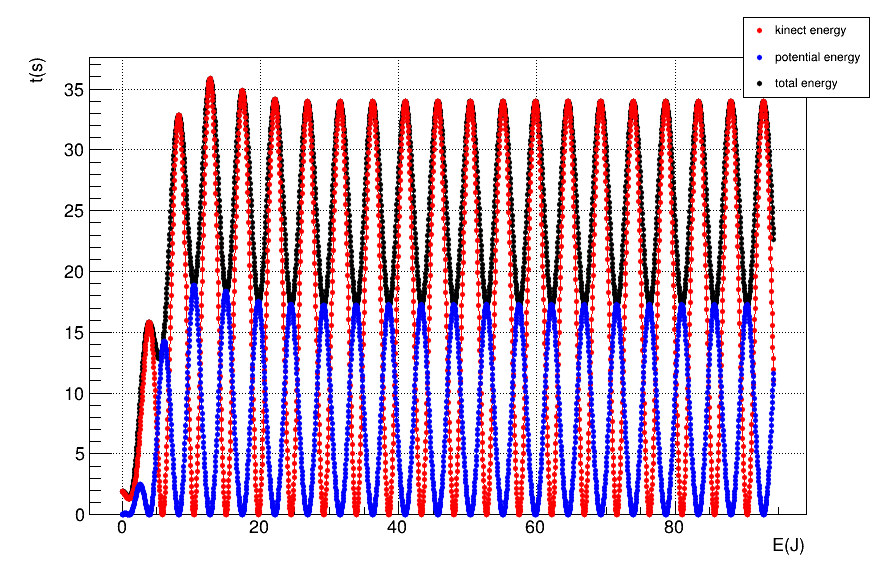
\includegraphics[scale=0.15]{../q2/alpha0.5/plots/Energies_t_RK.png}
% \end{center}

% \begin{center}
%     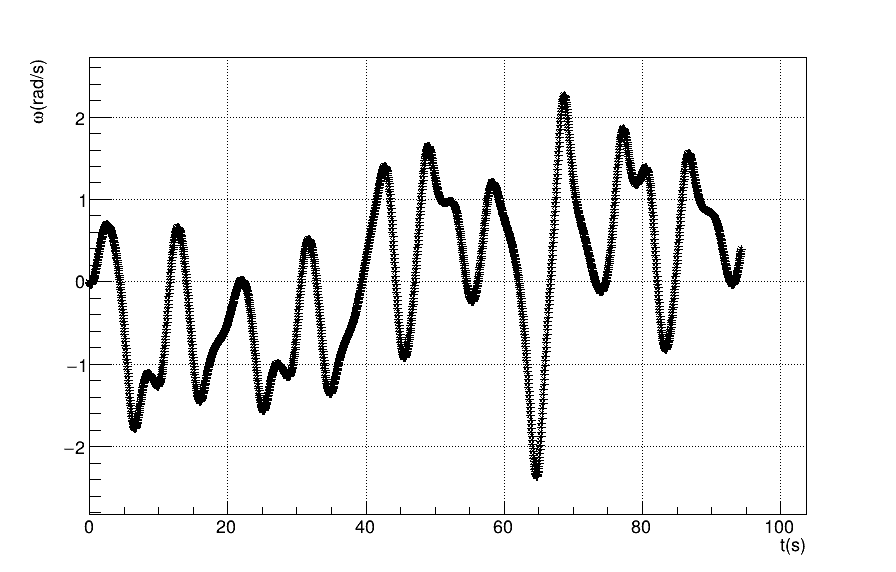
\includegraphics[scale=0.15]{../q2/alpha1.2/plots/omega_t_euler.png}
%     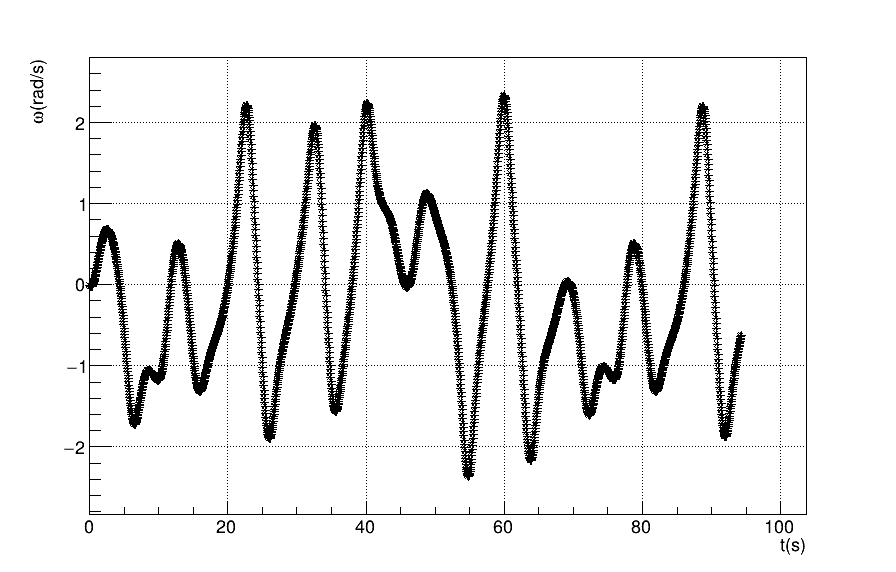
\includegraphics[scale=0.15]{../q2/alpha1.2/plots/omega_t_ec.png}
%     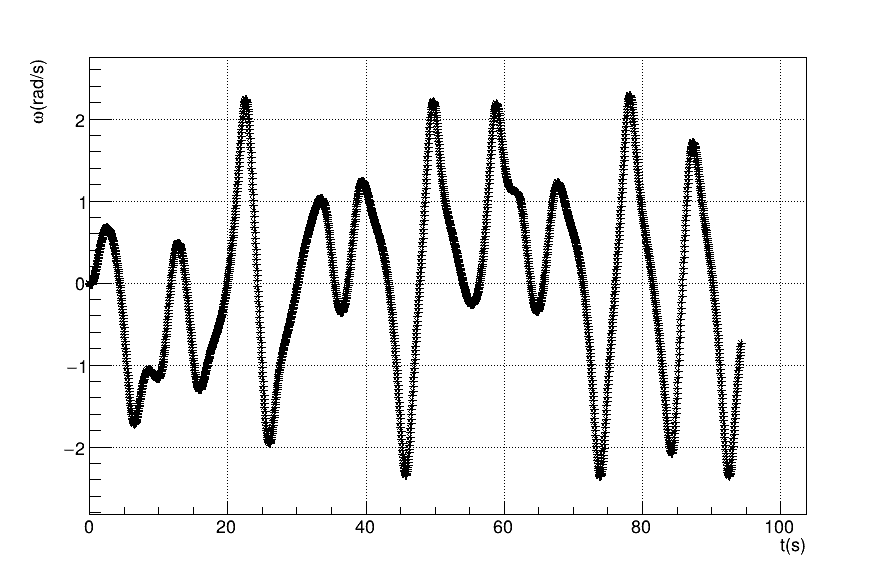
\includegraphics[scale=0.15]{../q2/alpha1.2/plots/omega_t_RK.png}
% \end{center}
% \begin{center}
%     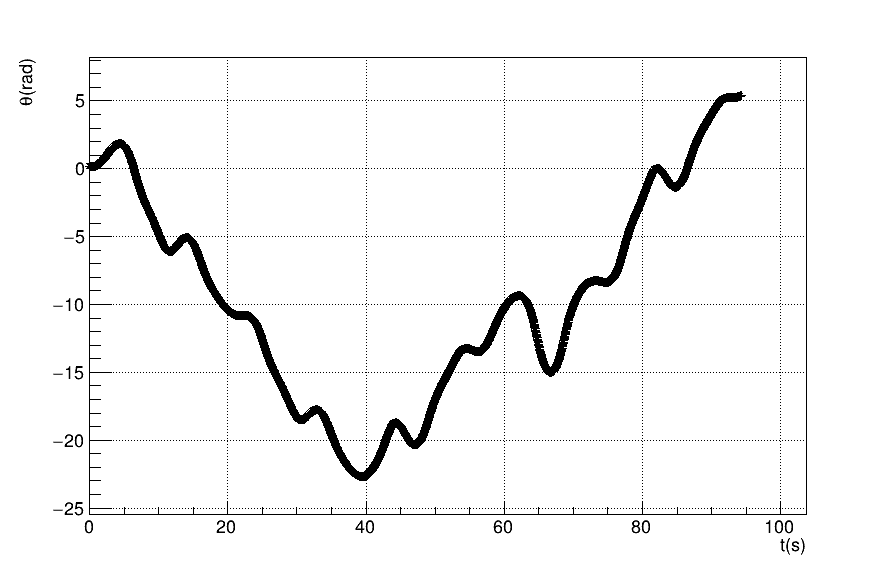
\includegraphics[scale=0.15]{../q2/alpha1.2/plots/theta_t_euler.png}
%     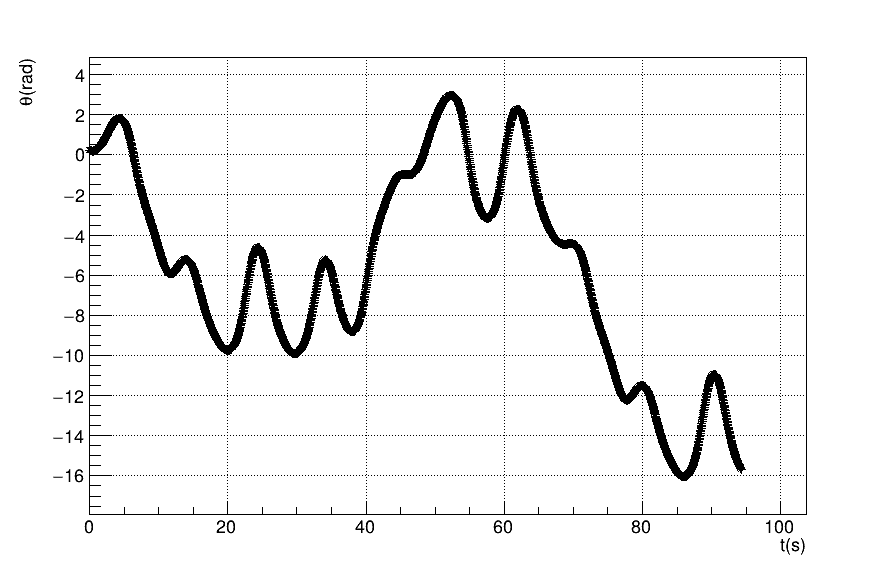
\includegraphics[scale=0.15]{../q2/alpha1.2/plots/theta_t_ec.png}
%     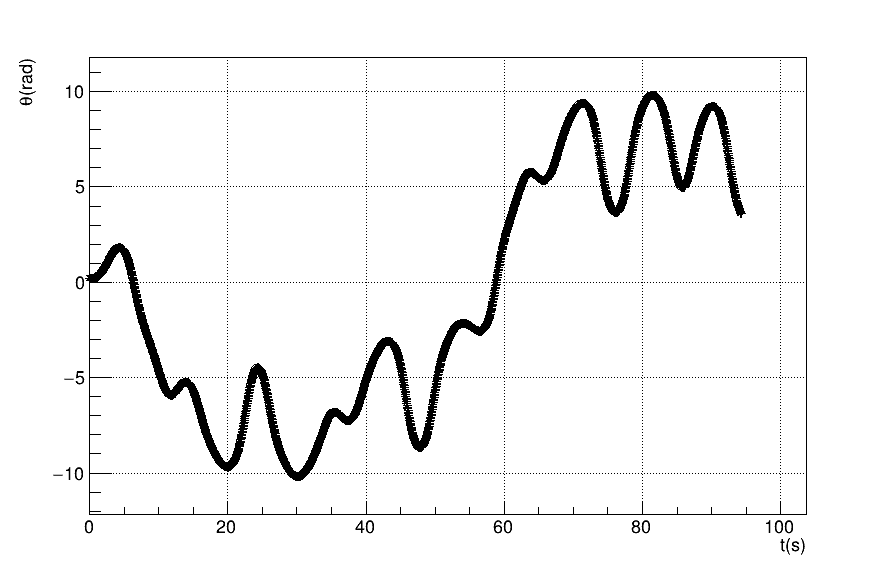
\includegraphics[scale=0.15]{../q2/alpha1.2/plots/theta_t_RK.png}
% \end{center}
% \begin{center}
%     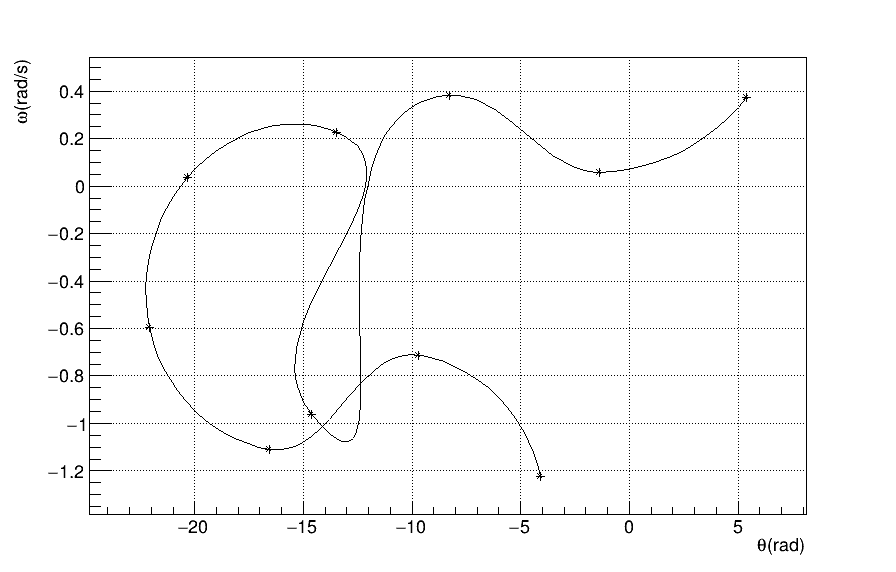
\includegraphics[scale=0.15]{../q2/alpha1.2/plots/poincare_euler.png}
%     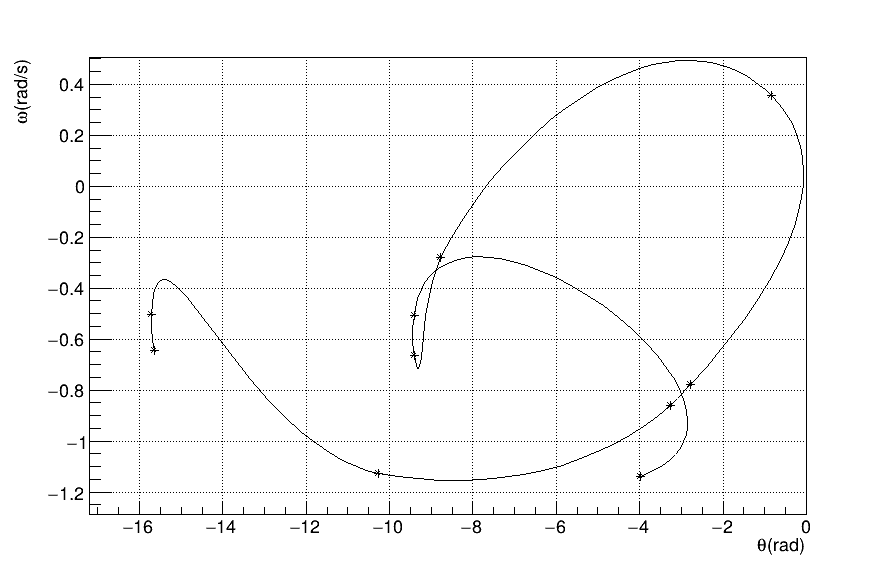
\includegraphics[scale=0.15]{../q2/alpha1.2/plots/poincare_ec.png}
%     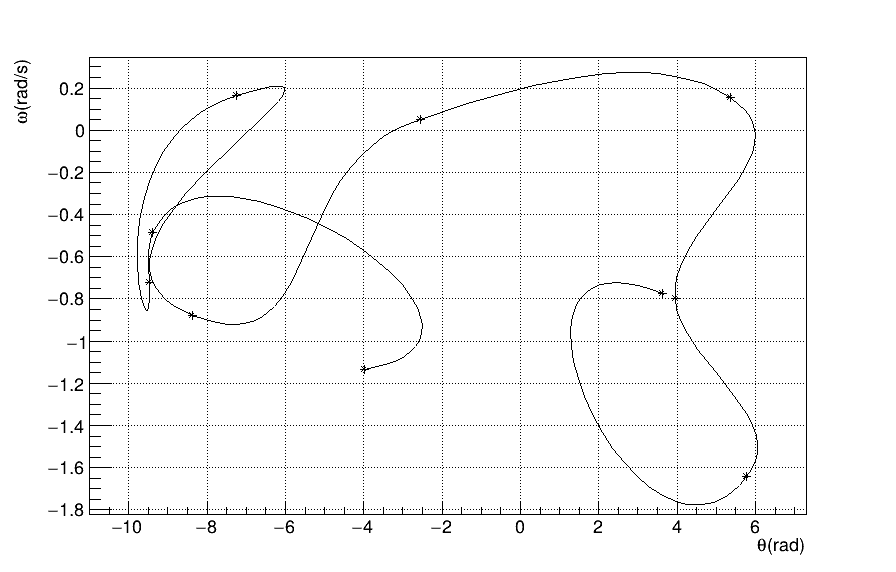
\includegraphics[scale=0.15]{../q2/alpha1.2/plots/poincare_RK.png}
% \end{center}
% \begin{center}
%     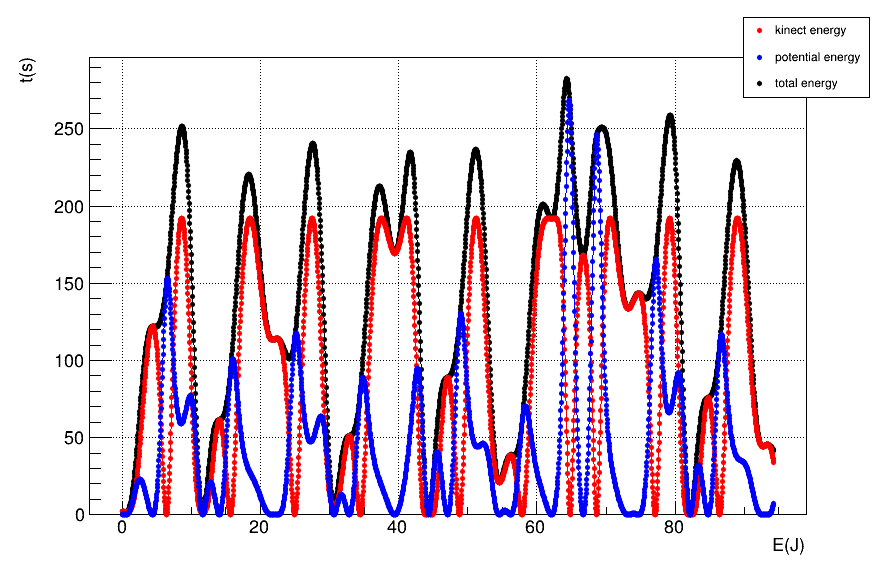
\includegraphics[scale=0.15]{../q2/alpha1.2/plots/Energies_t_euler.png}
%     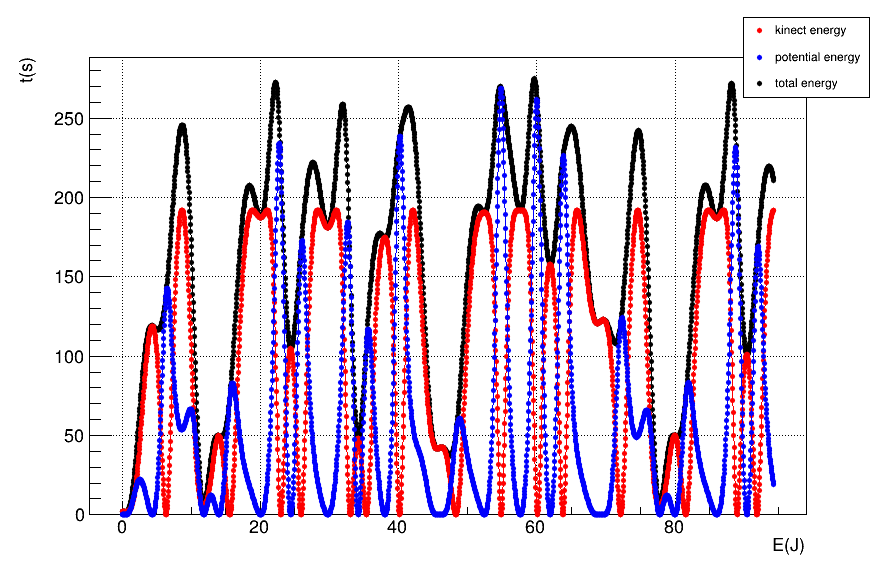
\includegraphics[scale=0.15]{../q2/alpha1.2/plots/Energies_t_ec.png}
%     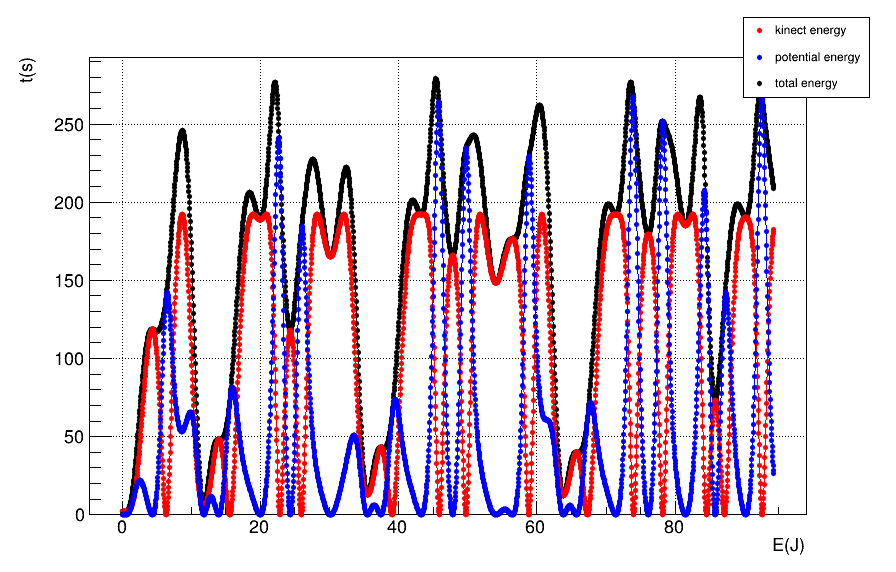
\includegraphics[scale=0.15]{../q2/alpha1.2/plots/Energies_t_RK.png}
% \end{center}

% \end{document}